\documentclass[nocopyrightspace,10pt]{sigplanconf}

\usepackage{url}
\usepackage{amsmath}
\usepackage{graphicx}

\newcommand{\todo}[1]{{\bfseries [[#1]]}}
%% To disable, just uncomment this line
\renewcommand{\todo}[1]{\relax}

\begin{document}
%
% --- Author Metadata here ---
%\conferenceinfo{CSE503}{'11 Seattle, USA}
%\CopyrightYear{2007} % Allows default copyright year (20XX) to be over-ridden - IF NEED BE.
%\crdata{0-12345-67-8/90/01}  % Allows default copyright data (0-89791-88-6/97/05) to be over-ridden - IF NEED BE.
% --- End of Author Metadata ---

\title{Real-time Code Clone Refactoring Recommendations}
% 1st. author
\authorinfo{Travis Mandel, Todd W. Schiller}
           {University of Washington}
           {\{tmandel,tws\}@cs.washington.edu}

\maketitle
\begin{abstract}
Code clone detection and analysis has historically been viewed as a
maintenance problem. Recently, tools for managing clones during
development have been introduced, however, these tools require
users to maintain formal clone models.
In this paper we propose a tool evaluation for (1) eliminating the
introduction of code clones during development without maintaining formal clone models, and (2) leveraging code
similarity to boost programmer productivity.

The tool
is an Eclipse plugin providing real-time clone detection and action
suggestions to the developer as (s)he writes and modifies
code. If time allows, machine learning will be 
employed to provide more pertinent results
and suggestions to the developer.
\end{abstract}

\category{D.2.6}{Software Engineering}{Programming Environments}

\keywords{refactoring, recommender system, code clones}

\section{Introduction}
\label{sec:intro}
Numerous studies suggest that code clones impair the maintainability
of software.

Yamashina et al. found in a sliding window analysis of a commercial CAD
application that 79.3\% of commits included modifications to files
containing code clones, but that only 9.7\% of such commits included
modifications to files containing the other
clones suggesting some clones may have erroneously not been updated
(the minimum clone length considered was 50 characters).
~\cite{Yamashina2008}. 
In a study of a commercial product line, Li and Ernst report that 4\%
of bugs were duplicated across at least one product or file;
additionally, they identified 282, 44, and 33 duplicated bugs in the
Linux kernel, Git, and PostgreSQL respectively~\cite{LiE2011}.

%Additionally, they report tenuous
%evidence from interviews and observation both novice and experience
%developers have difficuly finding code clones (the latter when
%identifiers have changed), and that novice developers do not
%systematically find all code clones before beginning to make
%revisions.

Under the assumption that code clones are not maintained properly,
Jeurgens et al. built a static bug detection tool based on
inconsistencies in clones, and confirmed that clones were a major
source of bugs in the study's subject programs~\cite{Juergens2009}.
Similarly, we hypothesize that when a developer (un)intentionally
nearly duplicates the functionality of an existing piece of code, without
referencing the original source, that the new code is more likely to
contain bugs than the original as it has not been tested or used in
production. Unifying code written by multiple developers has other 
benefits, such as improved code consistency, readability, and modularity.

Code clones have historically been viewed as a problem of software
\emph{maintenance}, as failure to revise a clone can be an error. 
Or, the task of identifying code clones is considered a separate and
independent development task, and thus may not be performed in a
manner consistent with eliminating bugs.

In addition to helping developers \emph{maintain} clones, this work
aims to help developers \emph{develop} more effectively by
facilitating actions in the presence of system clones, existing code
that is a (partial) clone of the source under development.  Our hypothesis
 is that identifying clones during development will prevent many of the problems
associated with duplicated code from ever arising, reducing development time.

The tool suggests two actions that eliminate code duplication:

\begin{enumerate}
  \item Replacing the code under development with a call to an existing method
  \item Extracting all, or part, of the system clone as a method;
    replacing the code under development with a call to the extracted
    method.
\end{enumerate}

\noindent Additionally, two actions may be suggested to help the developer
develop or maintain code with duplication:

\begin{enumerate}
\setcounter{enumi}{2}
  \item Aiding the user making analogous changes to the system clones
    by opening the relevant sections of code; 
    %, and potentially
    %supporting ``simultaneous editing''~\cite{Miller2002};
  \item Copying the system clone to the code under development,
    substituting identifiers as needed.
\end{enumerate}

Unlike other recent work for managing code clones during
development~\cite{deWit2009, Duala-Ekoko2007}, the tool does not
require the developer to manage a formal model of the clone linkages;
as the tool does not depend on explicitly tracked linkages, clones can
be identified as they are being developed to inform developer actions,
even if the developer does not perform a copy-paste action or
explicitly perform a clone search query.  We hypothesize many clones 
are written because the developer is not aware of preexisting functionality,
 so focusing only on copy-and-pasted clones
misses cases where functionality has been inadvertently 
duplicated.

This paper proceeds as follows: section~\ref{sec:finding-clones}
describes the user interface for the tool, along with the underlying
clone detectors. Section~\ref{sec:eval} proposes a controlled user
study to evaluate the tool. Section~\ref{sec:related} discusses
related work in clone detection, analysis, and refactoring. Finally,
Section~\ref{sec:conclusion} concludes.

\section{Finding Clones}
\label{sec:finding-clones}

% Don't use ``we'' to refer to the tool. The tool is the tool.

%As the programmer develops, the tool will analyze the code to
%determine the location of code clones, to aid in refactoring (method
%extraction), method calls, or copying. In the future, the tool could
%be extended to other refactorings / uses.

To support the developer actions enumerated in section~\ref{sec:intro},
the tool will search the existing codebase for code
that is similar to the region that is currently being developed or maintained
(i.e. where the cursor is). The search is performed using the clone detectors
described in section~\ref{sec:detectors}. The clone detection is implemented as
an Eclipse reconciler, which allows it to run in a background thread and only activate 
when there is a natural pause in typing.

In order to be practical in an online
setting with a large codebase, the detectors must be
fast and
robust to identifying clones that are more obfuscated than direct
copying, such as when a programmer re-implements the same
functionality.
%without referring to the first code section.

\subsection{Clone Detectors}
The tool is designed to perform detection both during development and
during maintenance.  As such, it may not be possible to parse the source
file, build an Abstract Syntax Tree (AST), or type the AST. Given this, text-based detectors
are advantageous because they can be run during active
development. When a program is parsable or compilable,
more-sophisticated detectors that use ASTs or program
dependence graphs ~\cite{LiE2011} produce better results
because they can use structural information when determining
similarity.

\label{sec:detectors}
The tool is currently packaged with three code clone detectors:

\begin{enumerate}
\item The Java Code Clone Detection (JCCD) API~\cite{JCCD}: performs
  AST-based similarity detection with support for a pipeline of AST
  operators; requires that the source files are parsable.
\item Checkstyle~\cite{CheckStyle}: performs a textual comparison on
  the lines of a program
\item Simian~\cite{Simian}: the Simian software is proprietary (though
  free for non-commercial use), but it appears the Simian can perform
  both textual and AST-based detection.
\end{enumerate}

All three detectors perform detection over the entire codebase, as
opposed to searching for clones for a given query. The speed of JCCD
and Checkstyle may not be practical for real-time detection in large
projects. Since both are open source, we can and will optimize the
detection for use in our tool, if necessary.  

These code clone detectors were selected because they all support Java
1.5 features (e.g., generics), are Java-based, and are freely
available for at least academic use. JCCD and Checkstyle are
open-source, and therefore can be modified to perform one-way clone
search. 
The tool is designed so that other clone detectors can be easily used instead.

%% TWS: the big-O analysis isn't correct, and I don't believe this adds anything
%% Such optimization could potentially involve exploiting knowledge of the 
%% modified code region to drastically reduce the complexity of the search,
%%  since instead of comparing all pairs of potential clones with $O(N^2)$, 
%% we would only need $O(N)$ comparisons to detect the clones. Currently, 
%% we only annotate clones located in the currently modified area, but
%% that is implemented as a filter instead of an algorithmic change.

%% We have been in contact with Li et al.~\cite{LiE2011} to apply program
%% dependence graph (PDG) approaches to clone search, however at this
%% time our search for a tool for generating detailed Java PDGs has been
%% unsuccessful.

Currently, only a single detector can be active at a time. In the
future, it may be beneficial to run the analyses simultaneously and
combine results.

\subsection{Displaying Suggestions}
\label{sec:display}
Clones \emph{with suggested actions} are displayed as Eclipse annotations,
which take 
the form of highlighting with a marker icon on the left vertical bar and a 
colored marking on the right vertical bar.  When users click the left marker,
the corresponding clone(s) and potential refactoring options are shown,
similar to Eclipse's QuickFix functionality for resolving errors and warnings.
Multiple clones at the same location are indicated by multicolored markers.
Figure \ref{fig:screenshot} shows the Eclipse Quick Fix interface.

\begin{figure}[here]
\centering
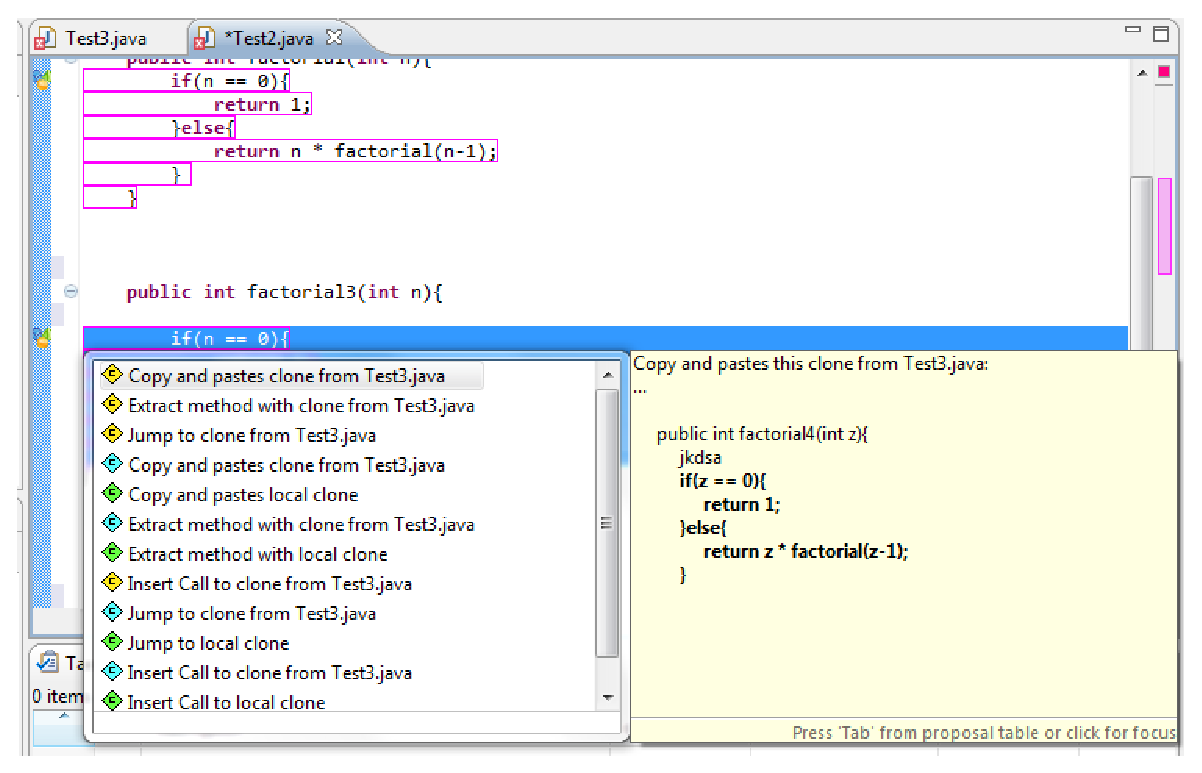
\includegraphics[width=80mm]{img/screen1.eps}
\caption{Eclipse Quick Fix clone suggestions. The color of the icon
  next to a fix differs by clone pair. The right side window shows the
  other side of the clone, higlighted with additional lines of
  context, or the body of the method call that will be inserted.}
\label{fig:screenshot}
\end{figure}

\subsection{Determining When to Make Suggestions}

Clone detectors score clone pairs based on code similarity; therefore,
the results may not be suitable for certains types of downstream
refactorings or other actions.
Additionally,
because we are presenting these clones to the user during development,
the suggestions must be conspicuous without being too obstrusive, lest
a developer disable the tool.
Our solution is to display conspicuous UI notifications
(see section \ref{sec:display}), while utilizing an 
adaptive scoring system to remove unhelpful UI elements based
on user actions.  

The tool determines a relevance for a clone pair and action according
to the following formula, which takes into account the user's previous
actions:

\begin{align*}
  Y = & \left[ X_{clone,action} * \left(\frac{B_{action}}{\sum{B}}\right) \right] \\
      & * (1-D)^{I_{clone}} * (1-M)^{N_{clone}}
\end{align*}

\noindent, where 
\begin{itemize}
  \item $Y$ is the adjusted relevance of the suggestion, which the
    Eclipse Quick Fix mechanism uses to order the suggestions (in
    practice, $Y$ is truncated such that $10 \le Y \le 100$,
    for this reason). Additionally, if $Y < T$, a fixed threshold, our
    tool excludes the suggestion from the set presented
    by Eclipse.
  \item $X_{clone,action}$ is an action-specific score for the clone
    determined by the clone pair's similarity, and a heuristic
    estimate of the usefulness of the action; calculation details
    are provided later in this section.
  \item $0 \leq B_{action}$ is the user's preference for the action; $B_{action} / 
    \sum{B}$ is the user's relative preference for the action. The
    initial values are set with normative information (e.g., it is
    better to insert a method call than it is to paste a clone). The
    value is then adaptively adjusted according to the users actions, as described
    later in section \ref{sec:preference}.
  \item $I_{clone}$ is the number of times one or more development
    actions occurred between Quick Fix sessions that included the
    clone (or since the clone was last included in a Quick Fix
    session).
  \item $N_{clone}$ is the number of times the clone has been
    displayed in a Quick Fix session
  \item $0 < D < 1$ is a constant ``development'' decay factor which
    reduces the suggestion's relevance under the assumption that when
    a user performs development taks between clone views, they have
    either (1) switched to another task, or (2) have explicitly
    determined not to act on clone's suggestions.
  \item $0 < M << D < 1$ is constant ``maintenance'' decay factor that
    reduces the clone's relevance when the developer ignores the
    clone's suggestions without performing development -- i.e., when
    the developer is exploring the code for maintenance purposes.
\end{itemize} 

In the current implementation, $X_{clone,action}$ is equal to the
similarity score determined by the clone detector, except for the
``insert method call'' action which is described in section~\ref{sec:call}.
Before performing the evaluation, we
plan to introduce action-specific factors for the other actions, e.g.,
how far away the other clone is in the code base for the ``extract
method'' and ``insert method call'' actions.

\subsubsection{Adapting to Developer Action Preferences}
\label{sec:preference}
When an action is selected in a Quick Fix session, the preference for
the action, $B_{action}$, is increased inversely with respect to its
distance from the threshold:

\begin{equation}
  B^{new}_{action} = B^{old}_{action} * \left[ 1 + \frac{100 - Y}{T} \right]
\end{equation}

\noindent, where $T$ is the threshold and 100 is the maximum allowable
score. If the user selects an action with a score close to, or at, the
threshold, it has a greater positive effect on the preference than
when the user selects a ``perfect'' action.
Time permitting, we also plan to investigate simple machine learning
strategies to base the preference term $B$ on the features of the
clone pair as well. The learner may
be trained on each individual user to
account for different programming styles.

\subsubsection{Scoring Method Calls}
\label{sec:call}
The score for an insert method call action for a clone is determined
from the (1) clone's similarity (2) the number of arguments in the
resulting method call, and (3) the percent of the method being called
that is covered by the clone:

\begin{equation}
  X_{action, clone} = S_{clone} * O * (1 - P)^N
\end{equation}

\noindent, where $S_{clone}$ is the similarity score for the clones, $O$ is
the percent of the callee that is covered by the clone, $0 < P < 1$ is a constant
penalty for the number of arguments in the resulting call, and $N$ is
the number of arguments in the resulting call. 

\section{Evaluation}
\label{sec:eval}

%We plan to evaluate based on user studies to determine how helpful our
%suggestions are.  Each user will be presented with an unfamiliar
%codebase and asked to implement a new method involving several We will
%record how many false positives there are, how many accepted
%suggestions there are, and how many times the user uses a method we
%extracted. We will record amount of code typed and amount of time
%spent. We will poll users after the fact to ask them how helpful they
%found the tool.

We will evaluate the tool via controlled user study. We will develop a fairly small 
Java codebase (15 files, 300 lines each) for this purpose. In addition to the code, the users will be
given a suite of JUnit tests which cover the codebase.  Most of the tests will pass
 on the provided code, 
but there will be several tests which test their development task and 
thus will not pass initially.  Our current idea is to have the codebase be part of an image processing library with a custom image format. (no visual rendering will actually occur) There will be a small set of classes in a separate package (such as the base image class) which the users will be instructed not to modify. Subjects will be instructed that they ``own'' all other classes in the code base, that is they have permission to introduce new methods, but must document the
methods.  

In the development portion of the study, the users will be then be directed
to implement a method of an existing class.     The subjects will be instructed to implement a method 
in such a way that the remaining unit tests pass.  They will be given a detailed 
 method specification. For example, the task may be to take a set of images and do a complex postprocessing operation them.  Implementing this specification will involve
 duplicating functionality that exists in other classes.  Some of the subtasks may be 
performed by static methods of the other classes, others may be performed 
within the body of methods belonging to the other classes. For example, blending images may be performed inside many methods, while reddening an image may be a separate function.
 Neither the specification
nor instructions will indicate that these clones exist.  We intend that, if the cloned parts of the 
task were replaced with method calls, the task would be about 5-10 lines, whereas duplicating clone functionality would take roughly 50 lines.

We will also include a maintenance task, as a second phase once the first is complete.  This task will involve functionality duplicated across the codebase.  We will provide each user with an initial location where the enhancement should occur.  For example, we will instruct the users that ``every time two images are blended, each should be darkened by 10\% first".  There will be 6 or so total locations that must be changed, but we will only tell users about the first one, and suggest that there might be others, but the total number will remain unknown to the user.

%\todo{Characterize the tasks and code base} 

The control group will use the stock Eclipse development
environment with logging code, the tool group will use the Eclipse development
environment with the tool. For the initial study for CSE 503, each
group will consist of two individuals who have experience using the
Java development environment.  


\subsection{Quantitative Evaluation}
For the development tasks, we will measure the time to complete the
task, the number of times the the tool detects a code clone throughout development (or would
detect a clone during development, for the control group),
the number of methods extracted/calls inserted, and the number of code clones
introduced into the code base, and percentage of the new code in the final method
 that is a duplicate (by human judgment) of other code. 
For the control group, we will additionally
record the number of times the developer searches for a method that
performs a subtask. 
For the tool group, we will record the number of
times the user ignores the tool's
alert, the user views the tool's analysis, and the user acts on the
tool's analysis. Additionally, when the user acts on the tool's
analysis, we will record the ranking of the clone the user acted on.  We expect to see a dramatic reduction in resulting method size and time (each approximately 50\% reduced).  We hope that the user views several of our suggestions and invokes the fixes several times.  Failure would be defined as the user never acts on any fix suggestion, and shows no significant reduction in code size or time spent on the task.

For the maintenance tasks, we will measure the time to complete the
task, and whether the user has correctly revised all of the clones. This will be measured
determined by a separate  hidden test suite, which is inaccessible to the 
users and will be run on their completed code only). 
We will record the same
group-specific metrics as for the development tasks.
We will be successful if the users with the clone tool correct significantly more of the duplicates than the control group and/or take significantly less time to fix the same number of duplicates.

\subsection{Qualitative Evaluation}
In addition to the quantitative results, we will have the study
participants respond to the following questions:

\begin{itemize}
  \item If you extracted a method, how did you decide to extract the
    method? 
  \item If you chose not to extract a method, why did you decide not
    to extract the method?
\end{itemize}

\noindent Additionally, the treatment group will respond to the following
questions:

\begin{itemize}
  \item Did you find the tool's suggestions helpful? If not, why?
  \item Was the ordering of the tool's suggestions valid? If not, why?
\end{itemize}

\subsection{Threats to Validity}
The evaluation outline in this section is meant as a preliminary study
to investigate the efficacy of the tool --- it is not meant to be
conclusive. That being said, this study, and potentially larger
studies of the same design have the following potential threats to
validity:

\begin{itemize}
  \item The study participants do not have to maintain the code in the
    future, and are therefore may be more likely to perform a
    short-sighted action
  \item The results may not generalize, as in real software there may
    be many de facto or de jure restrictions (e.g., a certain module cannot
    be changed) restricting the set of actions a user can make
  \item This tool seems especially helpful if it suggests that a
    developer is cloning code which that developer personally wrote in the
    past.  This is because the developer may not initially recall having written 
code with duplicate functionality and/or may not be willing to take the time to manually locate it,
but once the tool suggests the clone they may remember writing it and have no reservations about refactoring that section of code.
	If the tool suggests an unfamiliar section of code written by another developer, in constrast, the programmer may be less willing to refactor or otherwise modify it.
	Due to time limitations this scenario may be difficult to
    induce, as it usually occurs after one has been working on the
    same project for a long time.
\end{itemize}

We believe that the first threat can be mitigated via instructions to
the study participants. The second factor may require an additional
investigation where such restrictions are in place.  The third factor
requires a long-term study over weeks, months, or years.

\section{Related Work}
\label{sec:related}

The code clone literature can be divided into two areas: (1)
\emph{post} hoc code clone detection and
(2) \emph{development-time} clone management. By post-hoc we mean the scenario in which
detection is manually invoked to find all clones across an entire codebase, typically with the assumption that the codebase compiles and has already passed some level of testing.  In constrast, we use development-time to refer to the scenario in which detection automatically occurs as the user modifies code, typically without requirements about the compilability of the code.  The techniques used in the
post-hoc detection can vary greatly  based on the authors' definition of what 
level of similarity defines a ``clone", but typically utilize an
ad hoc model of clones. In contrast, the development-time literature focuses on
the creation and maintenance of formal code clone models during the
development process.

Roy et al provide a survey of post-hoc code clone detection
techniques~\cite{Roy2009}, and compares them by testing 
each on clones with varying levels of similarity. We do not wish 
to repeat the survey here, so we refer the reader to ~\cite{Roy2009}.
The rest of this section surveys the
related work on clone maintenance and refactoring, recommender systems,
development-time clone management, and \emph{development-time} code clone detection.

\paragraph{Post-hoc Clone Maintenance and Refactoring}

%TSM: I'm no longer certain why this belongs -- why just randomly pull out one of the 
% many post-hoc techniques?
%Visual Studio Ultimate contains a code clone detection tool andi
%interface; the tool can be run on a particular code fragment, or over
%the entire solution~\cite{VSClones}. 
%Other commercial products and
%academic artifacts exist which provide different interfaces /
%visualizations.

Several tools are similar to our work in that they attempt to not only
detect clones, but also provide refactoring techniques to eliminate the clones.  However,
they are post-hoc, so in contrast to our technique
 the detection and refactoring proposals are only presented once the 
programmer manually runs detection on a compiling codebase.

For example, Fanta and Rajlich propose a number of
potential refactorings for clones including function insertion, function encapsulation,
and method extraction \cite{Fanta1999}.  They 
present a case study for a C++ project which demonstrates that code refactoring is an important 
addition to clone detection. However, they do describe any way to rank or score the refactorings,
the programmer is required to choose based on code knowledge

Higo et al. present Aries, a tool which integrates various clone
information to present to the user \cite{Higo2008}.  The tool displays the
cloned blocks of code and presents refactoring options such as method
extraction; it augments the options with various metrics, including position in
the class hierarchy, and number of external variables. These metrics
are intended to help the programmer decide which refactoring, if any,
is appropriate. They do not, however, consider how to automatically 
propose the most helpful refactoring(s) based on these metrics, in contrast 
to our adaptive scoring system.

Kawaguchis et al. present a  
Microsoft Visual Studio interface for
displaying code clones in real-time to support software
\emph{maintenance} tasks~\cite{Kawaguchi2009,Yamashina2008}. Their
\textsc{Shinobi} system uses the CCFinderX's preprocessor and the Suffix Array
technique for indexing clones. Displayed clones are ranked via the sum
of the ratio files committed at the same time and the ratio of files
opened or edited at the same period in Visual Studio. Note that, unlike our tool,
 this sytem only \emph{displays} detected clones in real-time, detection is still
 a manual post-processing step.
%\todo{How do they get the latter piece of information?}

\paragraph{Development-time Clone Management}

From a user-interface stand-point, perhaps the work most similar to
ours is de Wit et al.'s \textsc{CloneBoard} Eclipse plugin that tracks
clone created by copy-paste operations~\cite{deWit2009}. Inspired
by~\cite{Mann2006}, the plugin registers code from copy-paste
operations as clones and prompts the developer with a set of actions
when the clone is modified: parameterize clone, unmark clone's tail,
unmark clone's head, postpone resolution, unmark clone, apply changes
to all clones, ignore changes. Inconsistent clones are identified via
a red marker on the left-column of the editor. Unlike our tool, only
clones arising from copy-paste operations are tracked, and the
developer explicitly manages the clone linkages.

Duala-Ekoko et al. present \textsc{CloneTracker}, an Eclipse plugin
for managing code clones that abstracts groups of clones via clone
region descriptors (CRDs) to track clones across software
versions~\cite{Duala-Ekoko2007}, a stark contrast toour ad-hoc model.
 The tool requires users to explicitly
create tracked clone groups by ``documenting'' a group of results from
the SimScan clone detection tool. \textsc{CloneTracker} additionally
supports simultaneously editing clones. However, in the author's
trials, the success rate of this feature to correctly modify the
clones was 80\%.

\paragraph{Recommender Systems}

Holmes and Murphy built the Strathcona tool for Eclipse which displays
relevant API usage examples when the developer performs a query by
selecting a region of code in the IDE; the search is based on the
structural content of the query line(s)~\cite{Holmes2005}. 
This is a similar interface to searching for clones in real-time, but a
much simpler process because only the API call must be matched.
Related systems also exist, but require the user to
perform a formal query, or to write special comments in the code.

\paragraph{Real-time Code Clone Search}

Applying code clone analysis during development places speed demands
on the detection algorithms. However, the need to only perform clone
detection in a single direction provides many opportunities for
speedup compared to traditional methods, which must search
over all pairs of potential clones.

Keivanloo et al. describe SeClone, a system for Internet code clone
search that performs clone pair clustering based on a ontology base on
features such as similarity~\cite{Keivanloo2011}. Similar to CCFinder,
it preprocesses files by generating the AST and abstracting the
tokens. The code patterns are used to quickly perform search, false
positives are limited by a retained set of type information. Results
are clustered via file-level type information.

Lee et al. introduce a method for instant structural code clone search
over large repositories by utilizing an R*tree indexing structure over
the characteristic vectors~\cite{Lee2010}.

Both \cite{Keivanloo2011} and \cite{Lee2010} only address finding the
clones quickly, and do not address locating possibly partial clones
during development, or presenting actions to the developer based on
the results.

\section{Conclusion}
\label{sec:conclusion}

In the past, code clones detection and analysis has been viewed as a
maintenance problem. 
We believe the problems code clones pose are 
more serious, namely that clones can cause disorganized code and
longer development time.
We have proposed a tool and evaluation for
eliminating the introduction of code clones during development, and
leveraging similar code to boost programmer productivity and improve
code robustness and organization.

%
% The following two commands are all you need in the
% initial runs of your .tex file to
% produce the bibliography for the citations in your paper.
\bibliographystyle{abbrv}
\bibliography{rt-refactoring-proposal,bibstring-abbrev,ernst,invariants,types}  % sigproc.bib is the name of the Bibliography in this case
% You must have a proper ".bib" file
%  and remember to run:
% latex bibtex latex latex
% to resolve all references
%
% ACM needs 'a single self-contained file'!
%
\end{document}
